\scanpage{24}
\mspage{11}

% top, rings one above the other
\[
\begin{aligned}
A_i^{\unsure{n|u}},B_i^n,C_i^n&\in\mathbb Z[\Lambda_0,\text{--},\Lambda_{n-1}]\\
&\hspace{3.2em}\cup\\
A_0^n,B_0^n,C_0^n&\in\mathbb Z[\Lambda_1,\text{--},\Lambda_{n-2}]
\end{aligned}
\]

% above NB, crossed line
\deleted{\unsure{Quand|Prenons} $\lambda_3=1$, \unsure{les autres} $\lambda_i$ $(i\geq4$}

% upper third, NB, uniqueness paragraph
\uline{NB} \unsure{Et.|Étt|Si} \inserted{\unsure{le polygone fixé, les} $u_i$ \unsure{(}$0\leq i\leq n-1$) \uline{et}} $\lambda_1\ \lambda_2\ \lambda_3$ fixés, \deleted{\unsure{ainsi que}} si de plus on suppose tous les \inserted{$u_i$ et les} $\lambda_i$ $(0\leq i\leq n-1)\ne0$, alors les $\lambda_i$ $(4\leq i\leq n-1)$ sont déterminés de façon unique. D'ailleurs la relation

% just above drawing
\[
\lambda_1u_0-\lambda_2(u_1+u_2)+\lambda_3u_3=0
\]

% middle right, beside drawing
montre que, si $u_0,\ u_1+u_2=u_1^3,\ u_3$ ne sont pas coll., alors les $(\lambda_1;\lambda_2,\lambda_3)$ possibles (pour cette relation) \unsure{font|forment} un espace de dim $1$, \unsure{resp.|i.e.} \deleted{\unsure{0}}.

% middle left
\figure{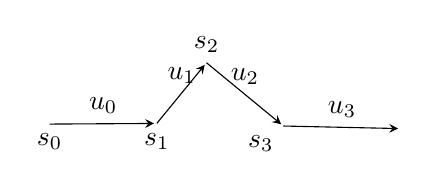
\begin{tikzpicture}[scale=.82,>=stealth]
\coordinate (a) at (0,0); \coordinate (b) at (1.66,.01); \coordinate (c) at (2.43,.95); \coordinate (d) at (3.62,-.03); \coordinate (e) at (5.44,-.07);
\foreach \p/\q/\i in {a/b/0,b/c/1,c/d/2,d/e/3}{\draw[->,shorten >=1pt] (\p)--(\q) node[midway,above] {$u_{\i}$};}
\node[below] at (a) {$s_0$}; \node[below] at (b) {$s_1$}; \node[above] at (c) {$s_2$}; \node[below left] at (d) {$s_3$};
\end{tikzpicture}}

% middle to lower part
$(\lambda_1,\lambda_2,\lambda_3)$ est \unsure{déterminé} mod \unsure{homothétie} par polygone -- donc aussi $(\lambda_0,\text{--}\lambda_{n-1})$. Changeant les rôles par \unsure{renumérotation|commutation|permutation}, on voit qu'il en est ainsi dès qu'il existe $i$, avec $u_i,\ u_{i+1}+u_{i+2},\ u_{i+3}$ non collin. Mais quand peut-on avoir \deleted{\unsure{les}} \unsure{vect.} coll $\forall i$ !

% lower right above coefficient calculations
\margin{OBS $u_0,u_1$ lin. indép.}

% foot, first pair of systems
\[
\begin{aligned}u_1+u_2&=-\alpha u_0\\u_3&=\beta u_0\end{aligned}
\qquad\left\{\begin{aligned}u_2&=-\alpha u_0-u_1\\u_3&=\beta u_0\end{aligned}\right.
\]

% foot, second pair and conclusions at right
\[
\begin{aligned}\deleted{\unsure{u_1|\alpha}}u_2+u_3&=\gamma u_1\\u_4&=\delta u_1\end{aligned}
\quad\text{i.e}\quad
\left\{\begin{aligned}u_3&=\alpha u_0+(1+\gamma)u_1\\u_4&=\delta u_1\end{aligned}\right.
\qquad\begin{aligned}\gamma&=-1\\\beta&=\alpha\end{aligned}
\]

% archive sheet number: 30
